These sensitivity studies are used to analyze parameters that are held constant during the simulations and determine if simplifications can be made to some with negligible impact on the results.
For these simulations, the parameters, unless otherwise specified, are given in Table \ref{tab:params-const}.

\begin{table}[H]
    \centering
    \begin{tabular}{lll}
        \hline
       Parameter  & Value & Units \\
       \hline
        OpenMC Batches & 10 & - \\
        OpenMC Particles & 50000 & - \\
        OpenMC Depletion Chain & ENDF/B-VIII.0 & - \\
        OpenMC Cross Sections & ENDF/B-VIII.0 & - \\
        Source Particles & $4.2\times 10^{16}$ & -\\
        Temperature & 920 & $K$\\
        Neutron Energy & $0.0253$ & $eV$\\
        Sample Nuclide & $^{235}U$ & -\\
        Sample Density & 10 & $\frac{g}{cm^3}$\\
        In-core Residence Time & 420 & $s$\\
        Ex-core Residence Time & - & $s$\\
        Irradiation Time & 420 & $s$\\
        Decay Time & 420 & $s$\\
        Decay Time Step & 1 & $s$\\
    \end{tabular}
    \caption{Default parameters used for sensitivity studies of constant parameters used in 0D flow \gls{DNP} group parameter formulation OpenMC simulations.}
    \label{tab:params-const}
\end{table}

OpenMC batches and OpenMC particles both refer to the settings in OpenMC which dictate the number of batches per generation and the number of particles per batch, respectively.
The source particles parameter dictates the strength of the neutron source.
The number of source particles is divided by the irradiation time to generate the neutron source rate used in OpenMC during the irradiation, as shown in Equation \eqref{eq:balancedsdot}.
The irradiation time is the amount of time the sample is irradiated, the decay time is the amount of time the sample has the delayed neutron count rate measured after irradiation, and the decay time step is the time step used when updating the nuclide concentrations post-irradiation.
Additionally, by default, no chemical removal is modeled.

\subsubsection{OpenMC Particles}

If this value can be reduced, then the total amount of simulation time can be reduced.
Alternatively, the default value may be insufficient for this problem and lead to inaccurate results.
The model is exceedingly simple, composed of only a small sphere of fissile material and a vacuum boundary condition.
Table \ref{tab:omc-nps} shows the total delayed neutron yields and average half-life for varying numbers of simulated particles in OpenMC.
Because more particles lead to a slower simulation, a balance must be found between accuracy and cost.
The differences between the largest number of particles for the total delayed neutron yield, $\bar{\nu}_d$, and the average half-life, $\bar{T}$, are given in the final two columns of the table.
Based on these values, 50000 particles results in a fit accurate for the average half-life and total yield while also being somewhat computationally inexpensive.


\begin{table}[H]
    \centering
    \begin{tabular}{rcccc}
Particles & $\bar{\nu}_d$ & $\bar{T}$ $[s]$ & $|\Delta \bar{\nu}_d|$ & $|\Delta \bar{T}|$ $[s]$ \\
\hline
1 & 0.016339 & 7.343276 & 0.002394 & 0.028612 \\
10 & 0.019469 & 7.313167 & 0.000736 & 0.001497 \\
100 & 0.018841 & 7.314828 & 0.000108 & 0.000164 \\
500 & 0.018810 & 7.314185 & 0.000077 & 0.000478 \\
1000 & 0.018693 & 7.315162 & 0.000040 & 0.000499 \\
5000 & 0.018667 & 7.314440 & 0.000066 & 0.000223 \\
10000 & 0.018700 & 7.314947 & 0.000033 & 0.000284 \\
50000 & 0.018741 & 7.314586 & 0.000008 & 0.000077 \\
100000 & 0.018730 & 7.314608 & 0.000002 & 0.000055 \\
500000 & 0.018731 & 7.314636 & 0.000002 & 0.000028 \\
1000000 & 0.018733 & 7.314663 & - & - \\
    \end{tabular}
    \caption{Sensitivity study of total delayed neutron yields and average half-lives due to number of particles simulated in OpenMC.}
    \label{tab:omc-nps}
\end{table}

The variation in these values for lower particle counts is driven by differences in the group 2, 3, and 4 fits.
Figure \ref{fig:yields-nps} shows the group yields for each different number of particles, where the largest differences are in groups 2, 3, and 4.
These group half-lives range from 4.4 to 24 seconds.
The cause of this difference must be from differences in nuclide concentrations post-irradiation, as the emission probability and decay constant data are the same between the different simulations compared here.
To evaluate which nuclides are causing this difference, the standard deviation of each set of concentrations is divided by the mean, which results in the \gls{CV} for each nuclide.
Some of the nuclides with the largest \gls{CV} have a negligible contribution to the delayed neutron yield, such as $^{209}Tl$.
To scale by this consideration, the \gls{CV} is multiplied by the total number of delayed neutrons emitted from that nuclide $i$, $\bar{\nu}_{d, i}$, the equation for which is given in Equation \eqref{eq:delnu-net-nuc}, replicated here:

\begin{equation}
    \bar{\nu}_{d, i} = P_{n, i} \lambda_i N_{i, 0}
    \nonumber
\end{equation}


\begin{figure}[H]
    \centering
    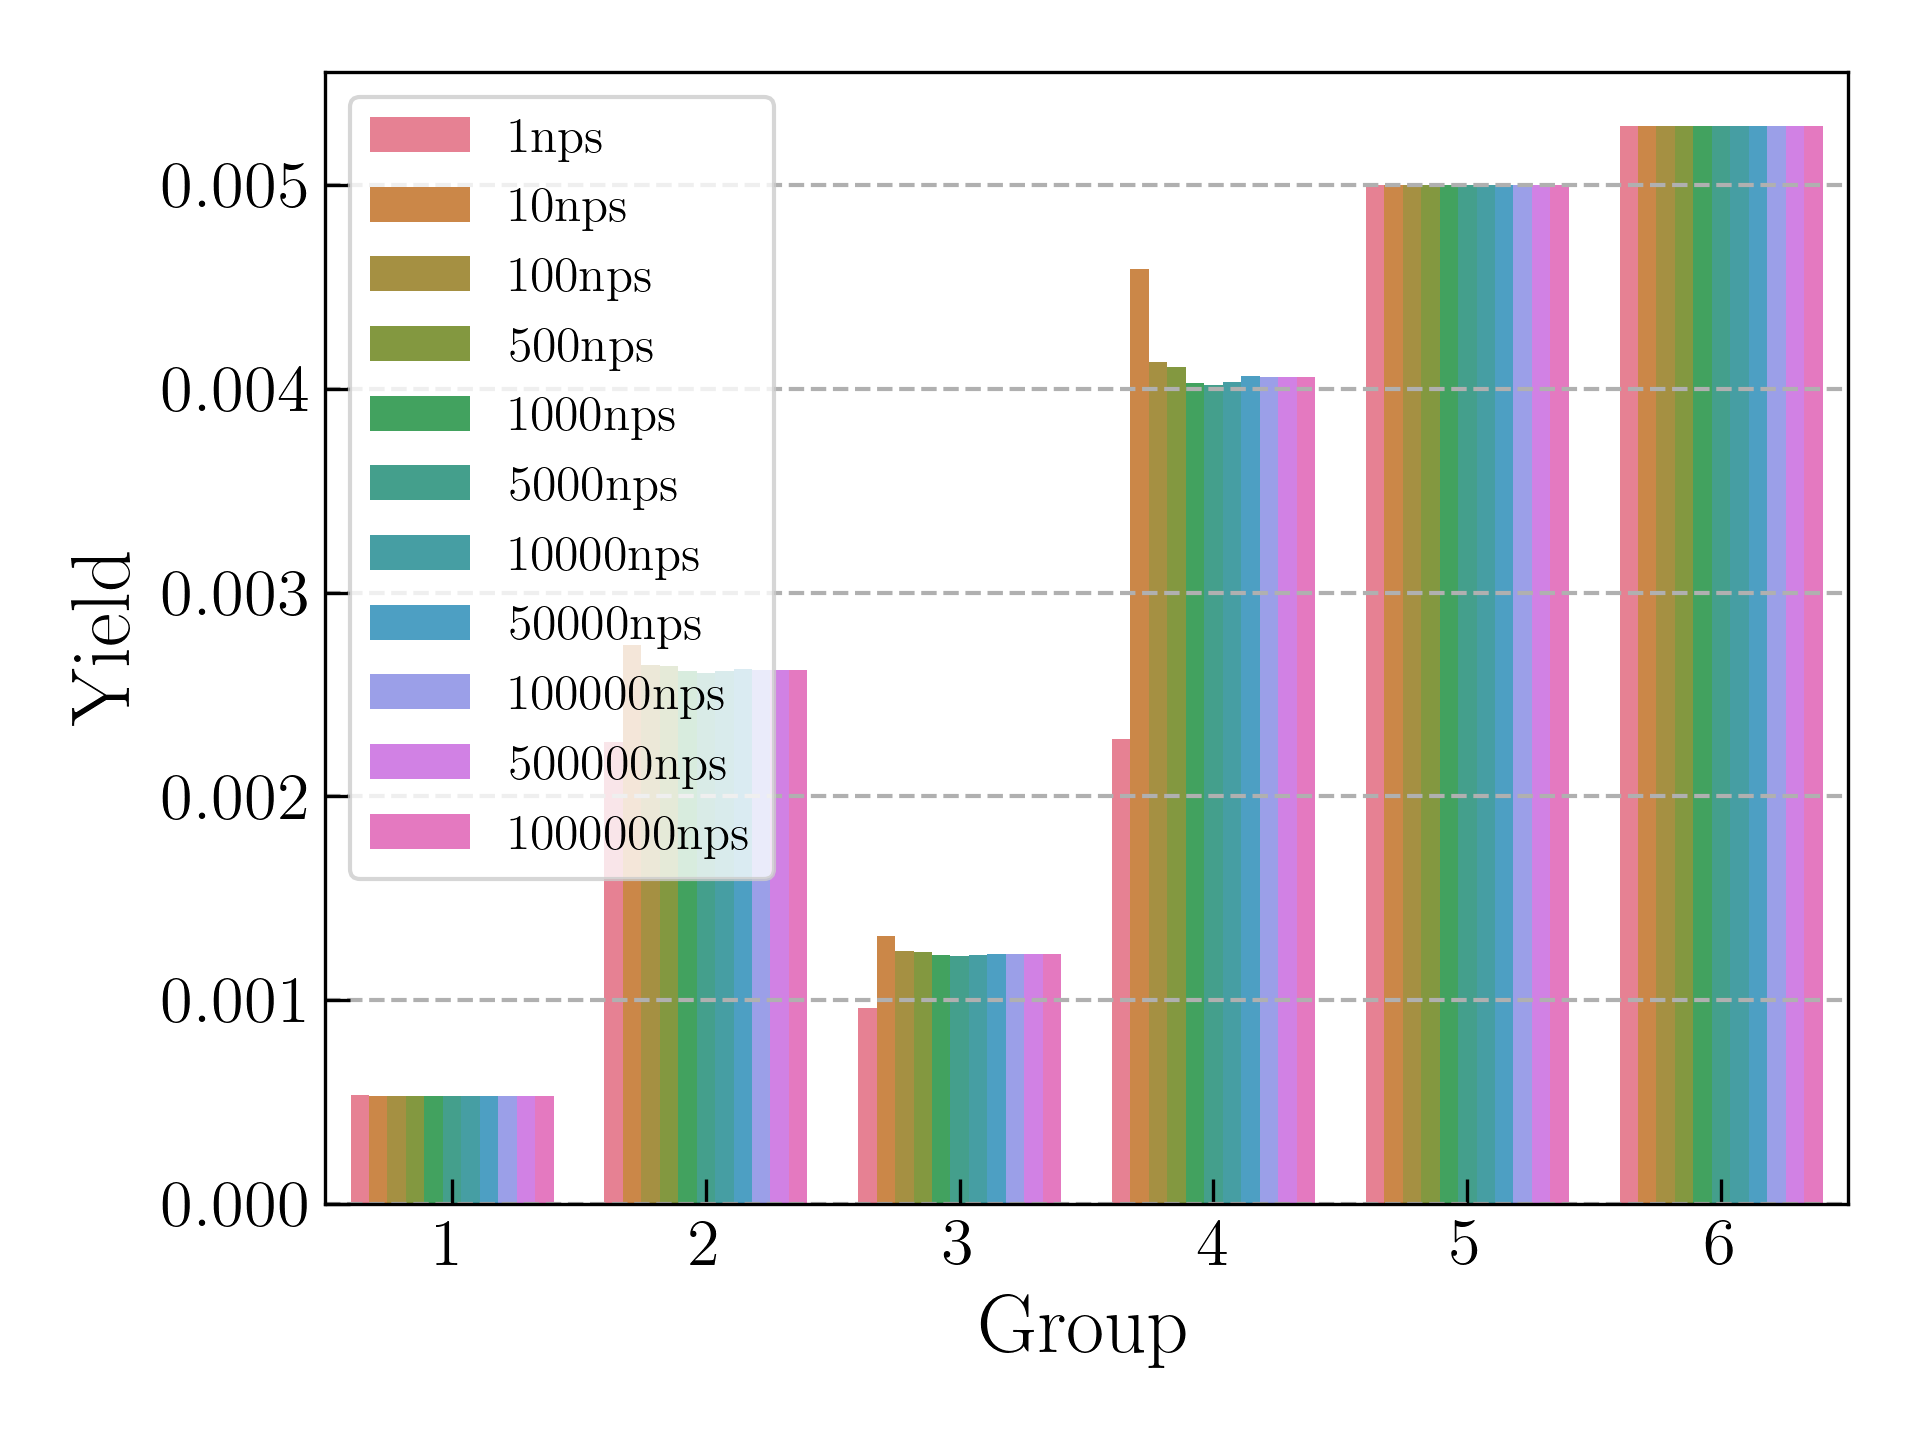
\includegraphics[width=\linewidth]{images/yields-csvs-nps.png}
    \caption{Group yields resulting from various numbers of simulated particles in OpenMC.}
    \label{fig:yields-nps}
\end{figure}

The scaling of the \gls{CV} by the total delayed neutron yield is important because nuclides like $^{209}Tl$ have a \gls{CV} of 9.65\%, but a total delayed neutron yield of 0.
The nuclides are sorted by a new scoring term, $\alpha$, where the full term in Equation \eqref{eq:sorting-term} is given as:

\begin{equation}
    \alpha_i = \frac{\bar{\nu}_{d, i} CV}{\bar{\nu}_{d}}
    \label{eq:sorting-term}
\end{equation}

Based on $\alpha$, only two of the top ten nuclides are within groups two through four, with the nuclides being $^{89}Br$ and $^{137}I$.
When sorting by \gls{CV} instead, none of the top thirty nuclides are within groups two through four.
If the \gls{CV} is replaced with the standard deviation, then there are six out of ten nuclides which are withing groups two through four.
These nuclides are $^{137}I$, $^{88}Br$, $^{93}Rb$, $^{89}Br$, $^{138}I$, and $^{136}Te$.
Although the relative changes in these nuclides are smaller, the absolute change is larger, which drives a greater difference in groups 2 through 4.

\subsubsection{Temperature}

\begin{figure}[H]
    \centering
    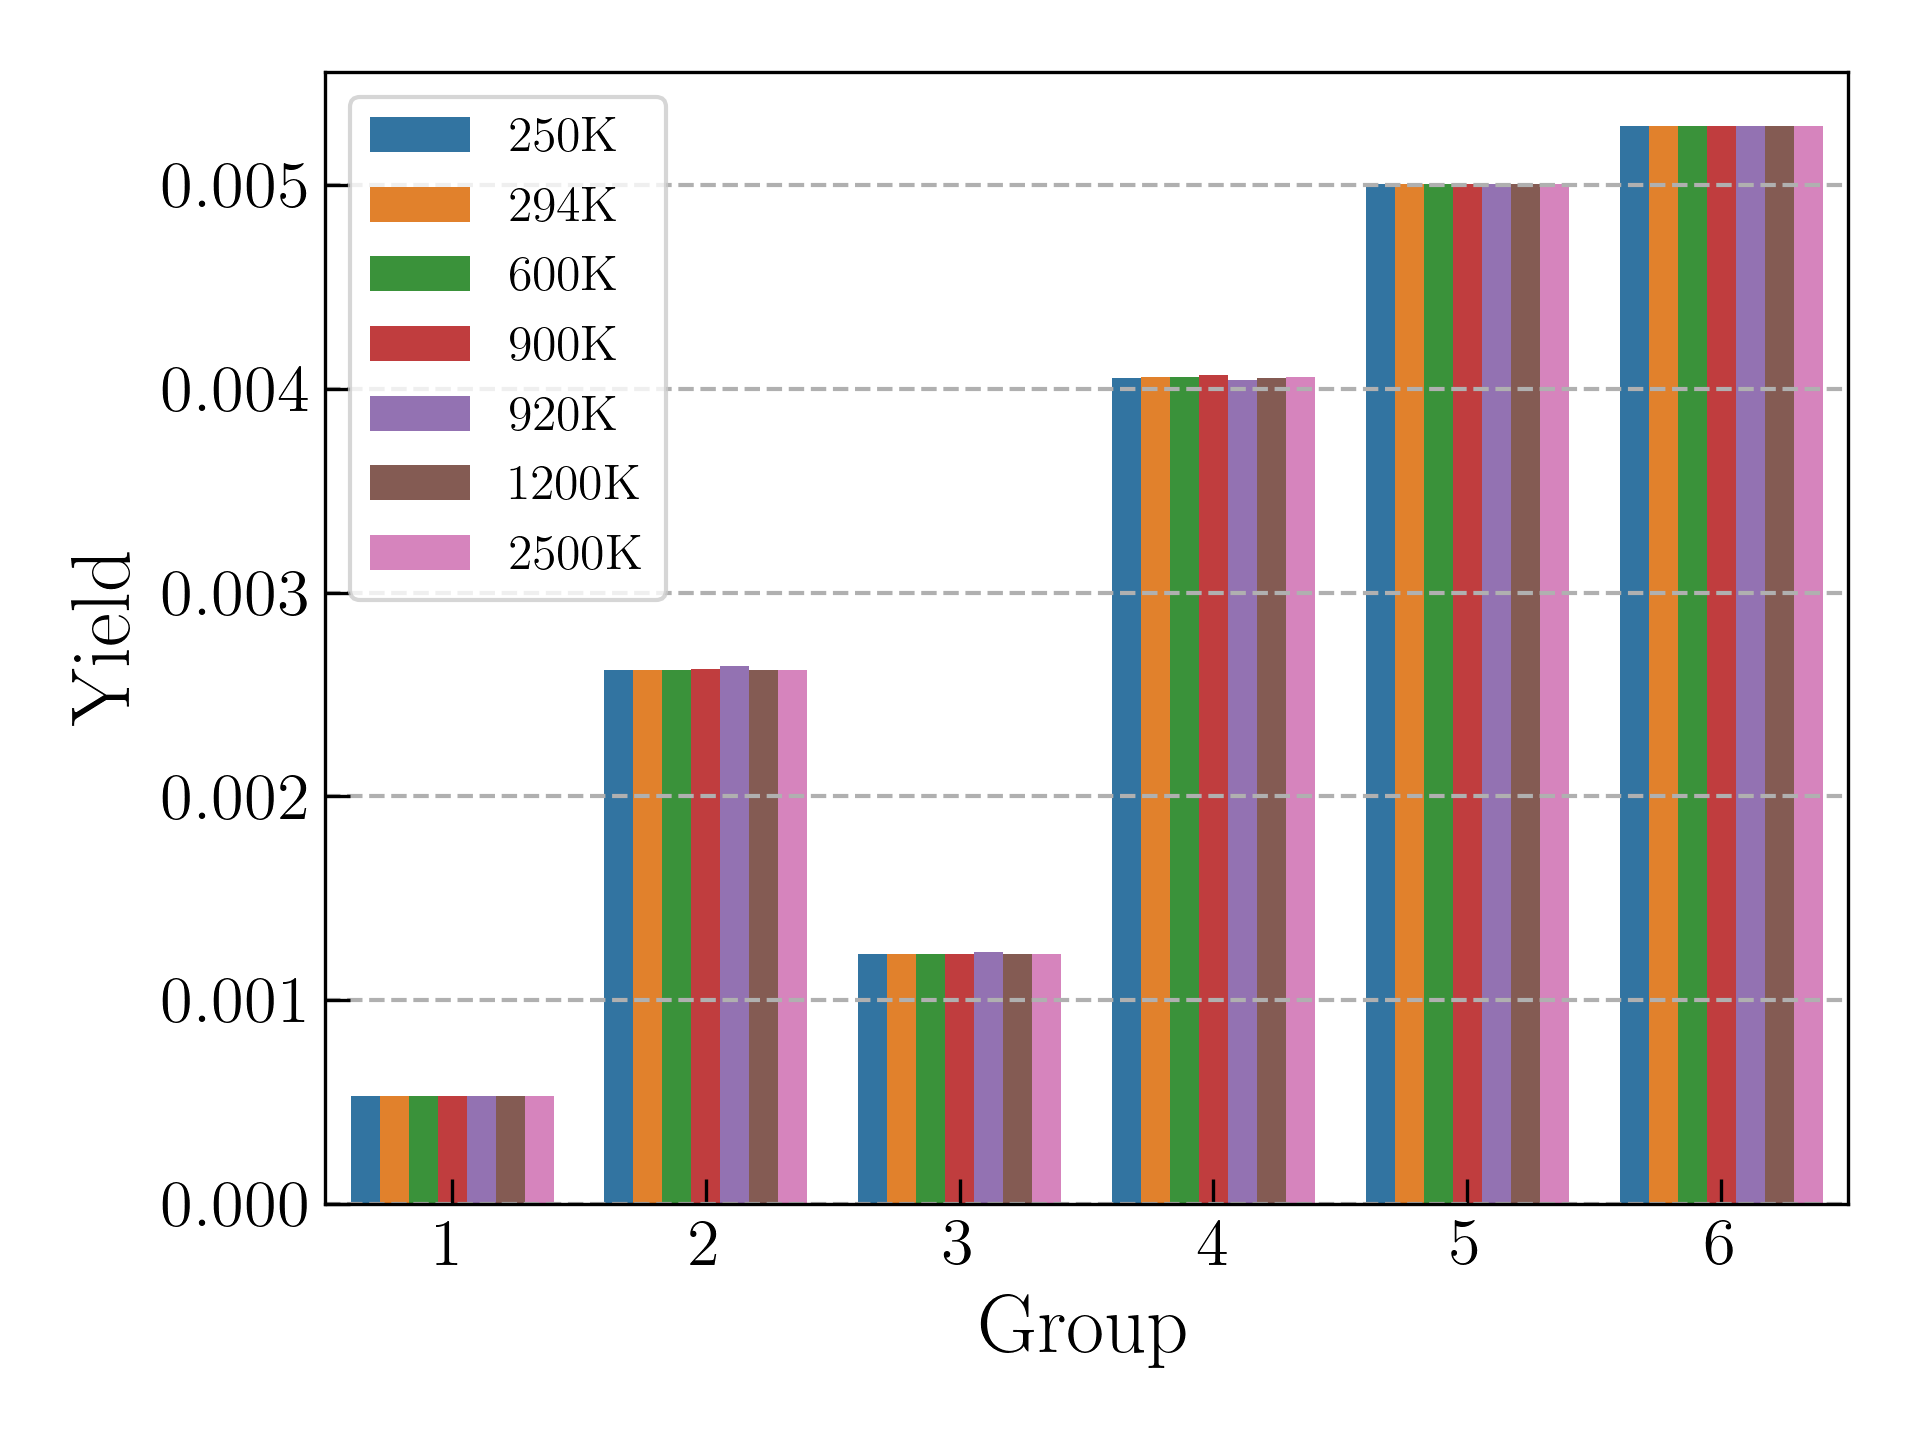
\includegraphics[width=\linewidth]{images/yields-csvs-K.png}
    \caption{Group yields resulting from various sample temperatures in OpenMC.}
    \label{fig:yields-K}
\end{figure}

\begin{table}[H]
    \centering
    \begin{tabular}{rcccc}
Temperature $[K]$ & $\bar{\nu}_d$ & $\bar{T}$ $[s]$\\
\hline
250 & 0.018729 & 7.315157 \\
294 & 0.018732 & 7.314929\\
600 & 0.018735 & 7.314949 \\
900 & 0.018743 & 7.314833 \\
920 & 0.018745 & 7.318251\\
1200 & 0.018722 & 7.314862 \\
2500 & 0.018732 & 7.315089 \\
    \end{tabular}
    \caption{Sensitivity study of total delayed neutron yields and average half-lives due to the sample temperature simulated in OpenMC.}
    \label{tab:omc-tirrad}
\end{table}

\subsubsection{Target Density}

\begin{figure}[H]
    \centering
    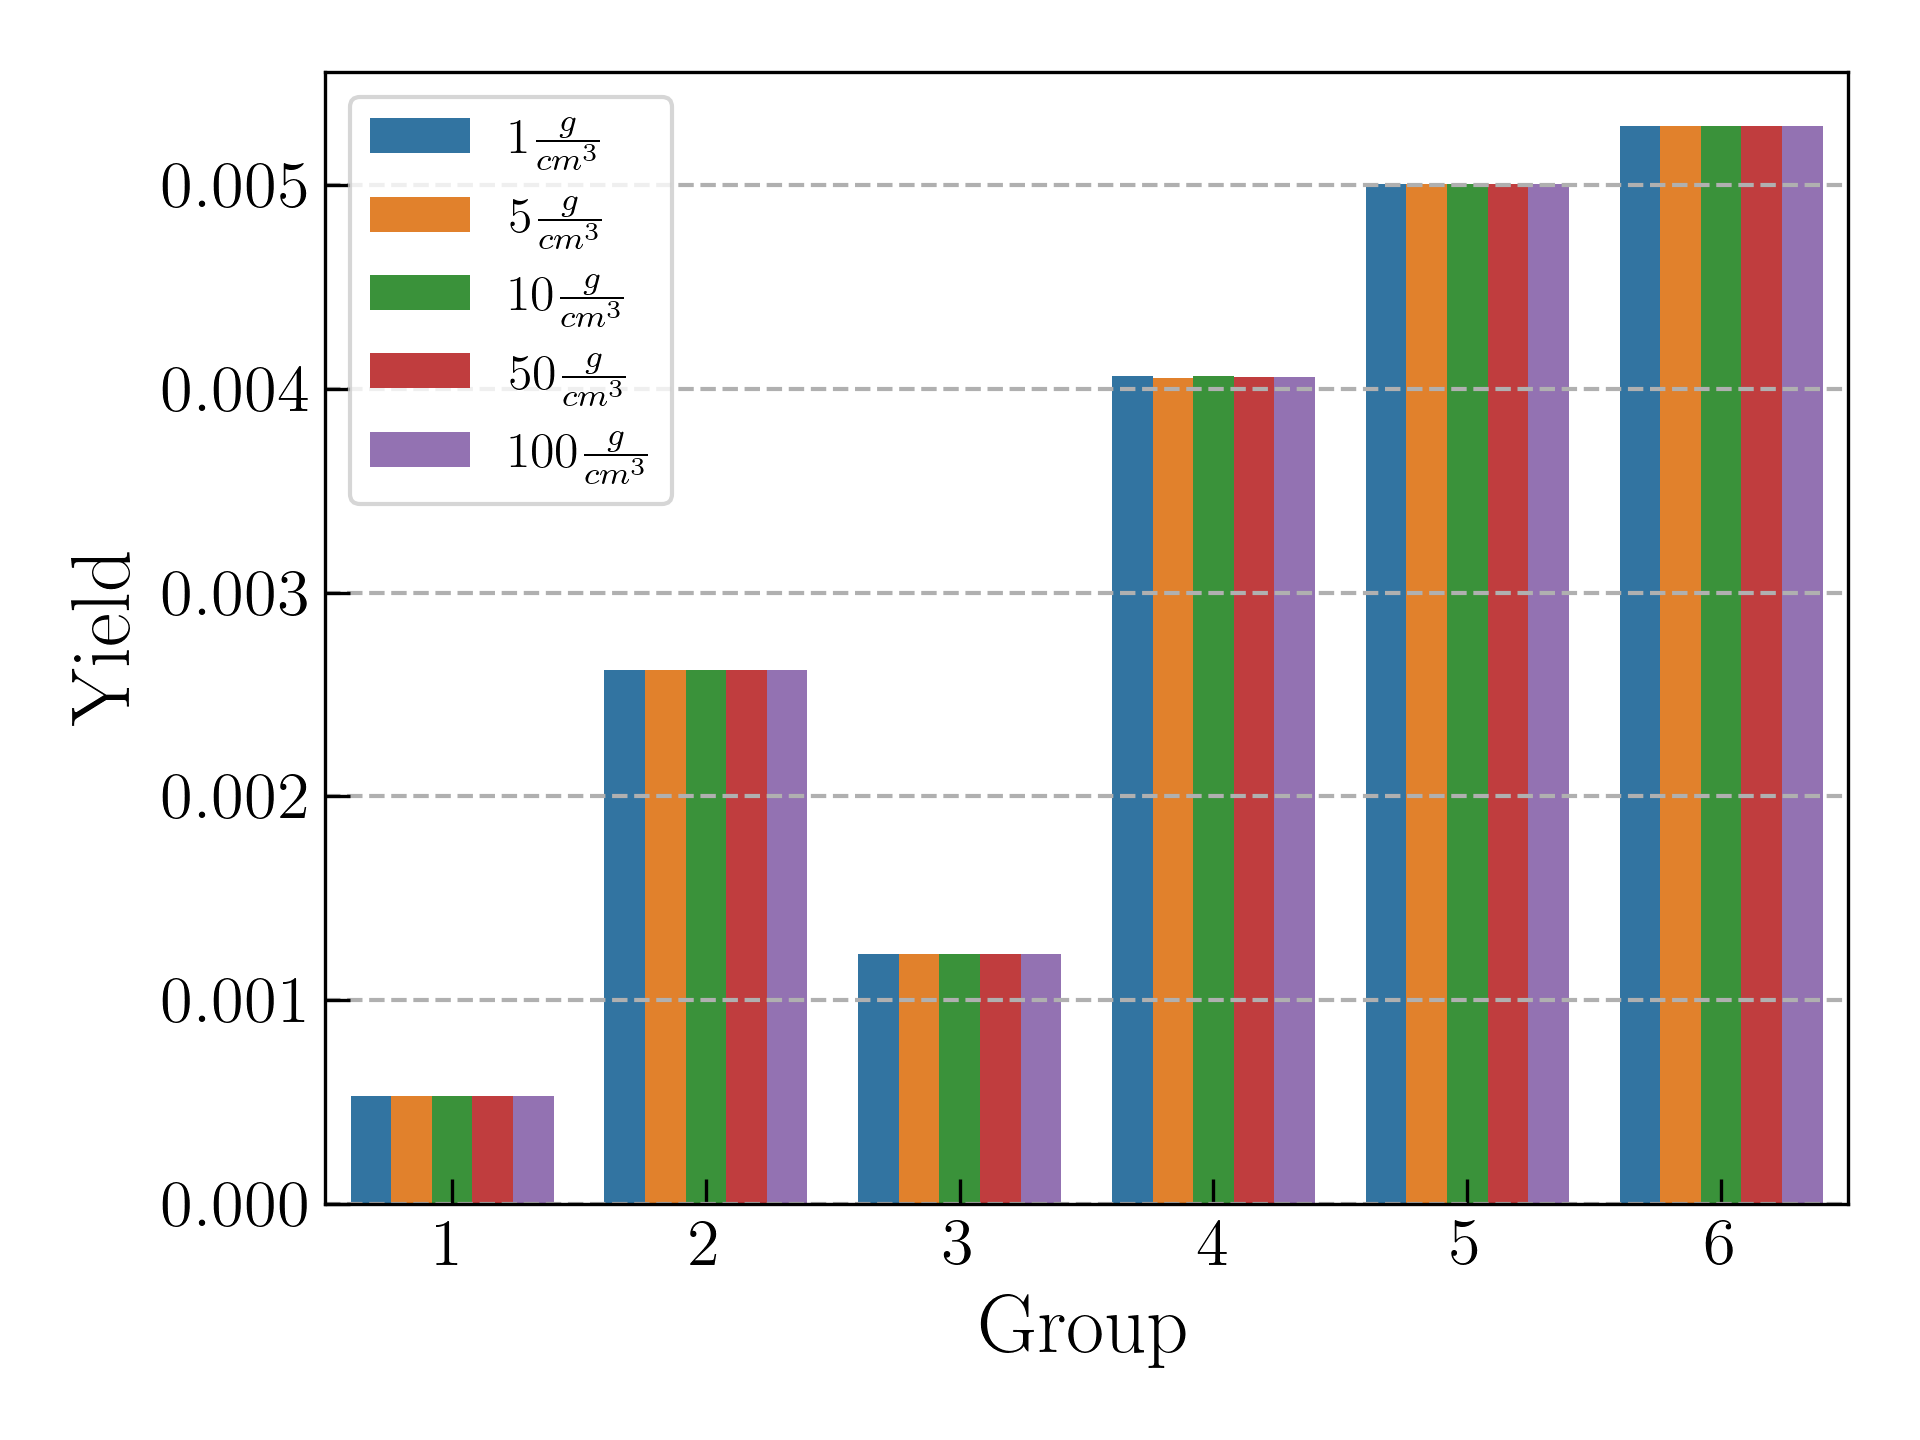
\includegraphics[width=\linewidth]{images/yields-csvs-gpcc.png}
    \caption{Group yields resulting from various sample densities in OpenMC.}
    \label{fig:yields-gpcc}
\end{figure}

\begin{table}[H]
    \centering
    \begin{tabular}{rcc}
Density $[\frac{g}{cm^3}]$ & $\bar{\nu}_d$ & $\bar{T}$ $[s]$ \\
\hline
$1$ & 0.018738 & 7.313331\\
$5$ & 0.018725 & 7.313464\\
$10$ & 0.018735 & 7.313371\\
$50$ & 0.018731 & 7.313418\\
$100$ & 0.018730 & 7.313413\\
    \end{tabular}
    \caption{Sensitivity study of total delayed neutron yields and average half-lives due to sample density simulated in OpenMC.}
    \label{tab:omc-gpcc}
\end{table}




\subsubsection{Irradiation Time}

\begin{figure}[H]
    \centering
    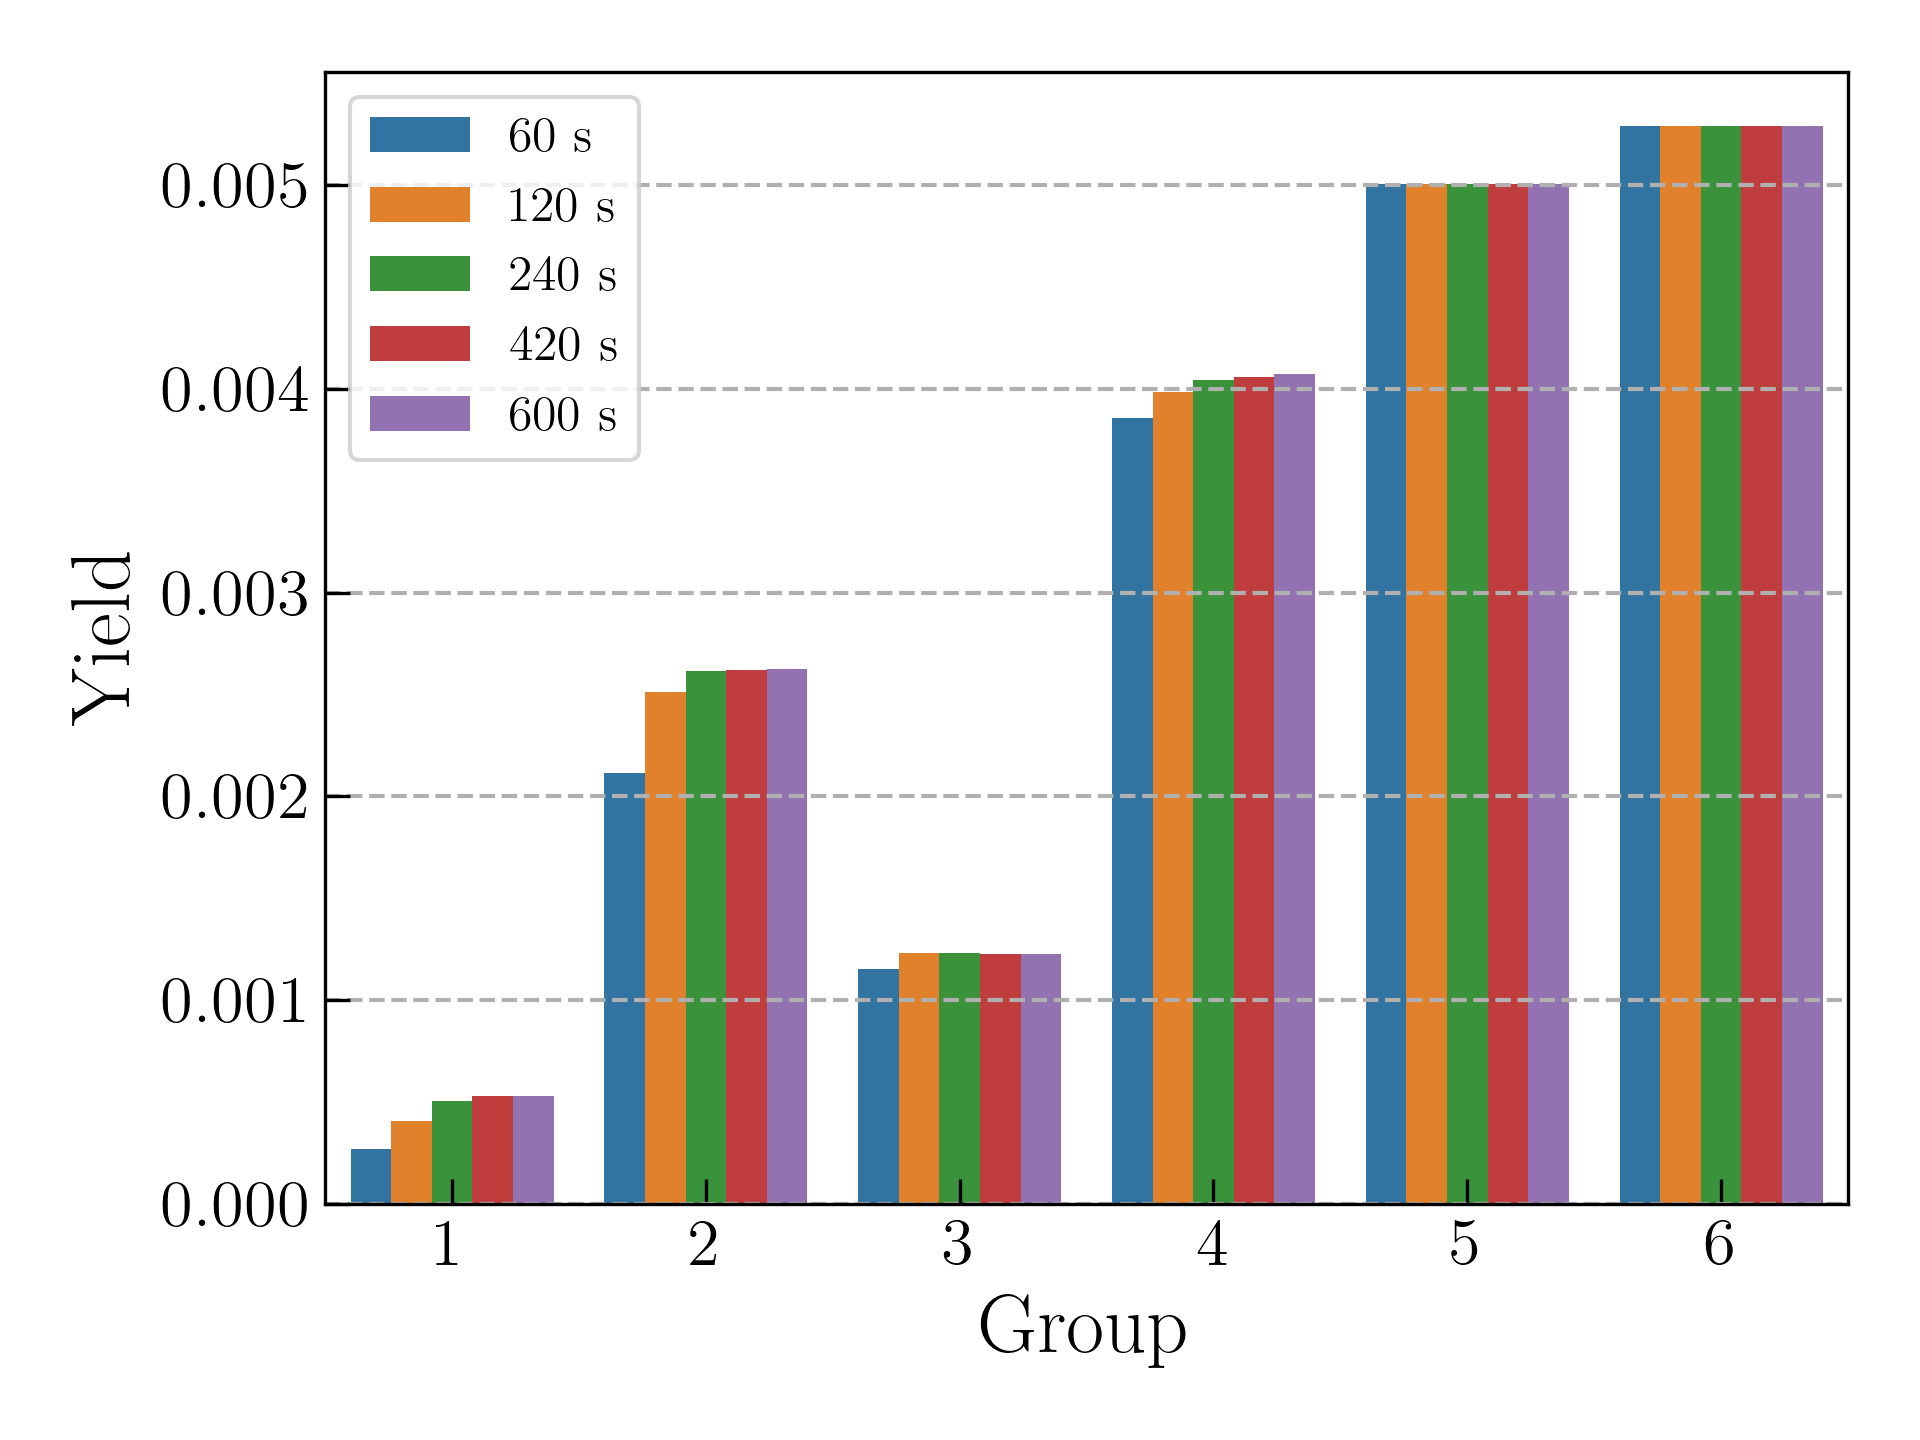
\includegraphics[width=\linewidth]{images/yields-csvs-tirrad.png}
    \caption{Group yields resulting from various irradiation times in OpenMC.}
    \label{fig:yields-tirrad}
\end{figure}

\begin{table}[H]
    \centering
    \begin{tabular}{rcccc}
Time $[s]$ & $\bar{\nu}_d$ & $\bar{T}$ $[s]$ & $|\Delta \bar{\nu}_d|$ & $|\Delta \bar{T}|$ $[s]$ \\
\hline
60 & 0.017690 & 7.388026 & 0.001062 & 0.066482 \\
120 & 0.018433 & 7.355979 & 0.000319 & 0.034434 \\
240 & 0.018687 & 7.329571 & 0.000065 & 0.008026 \\
420 & 0.018731 & 7.322325 & 0.000021 & 0.000780 \\
600 & 0.018752 & 7.321545 & - & - \\
    \end{tabular}
    \caption{Sensitivity study of total delayed neutron yields and average half-lives due to net irradiation time simulated in OpenMC.}
    \label{tab:omc-tirrad}
\end{table}


\subsubsection{Decay Time and Decay Time Steps}
\label{sec:time-eval}
The bulk of the computational cost comes from writing statepoint files; sufficient resolution is required to ensure a smooth decay curve.

\subsubsection{Large Cycle Time Elements}
\label{sec:large-tcyc}

%\subsubsection{Refuel Rate}
%\label{sec:ref-rate}

\subsubsection{Decay Daughter Tracking}
\label{sec:decaychaindaughters}
